\documentclass[]{article}

\usepackage{graphicx}
\usepackage{float}

\usepackage{amsmath}
\usepackage{amssymb}
\usepackage{amsthm}
\usepackage{xspace}

\newtheorem{theorem}{Theorem}[section]
\newtheorem{algorithm}[theorem]{Algorithm} %{\bfseries}{\itshape}
\newtheorem{lemma}[theorem]{Lemma}
\newtheorem{note}[theorem]{Note}
\newtheorem{proposition}[theorem]{Proposition}
\newtheorem{corollary}[theorem]{Corollary}

\newenvironment{definition}[1][Definition]{\begin{trivlist}
\item[\hskip \labelsep {\bfseries #1}]}{\end{trivlist}}
\newenvironment{example}[1][Example]{\begin{trivlist}
\item[\hskip \labelsep {\bfseries #1}]}{\end{trivlist}}
\newenvironment{remark}[1][Remark]{\begin{trivlist}
\item[\hskip \labelsep {\bfseries #1}]}{\end{trivlist}}

\newcommand{\Oo}{\mathcal O} %big-O notation
\newcommand{\oo}{\mathcal o} %small-O notation ;)

\newcommand{\funk}[1]{\small\texttt{#1}}
\newcommand{\cpp}{C+\!+\xspace}

\title{Hashing for variable length strings}
\author{Thomas Laumann Jespersen \and Eva Rotenberg}

\begin{document}
\maketitle

We use polynomial string hashing to obtain universal hashing of strings of variable length.

For fixed length strings, some very fast hashing functions exist, but for variable length strings, so far no version of "multiply shift" has been developed. 

However, one can divide the string into chunks of fixed length, use a very fast hashing function on each chunk, and apply the universal hashing function on the result, which again has variable length. We call this "wrapped polynomial string hashing" as opposed to "direct polynomial string hashing".

The obtained result is a fast \emph{universal hash-function} for strings of unbounded length. %, which performs better in practice than the standard library implementation. 
%TODO: Bedre end std lib?

\section{Theory}

\subsection*{Direct polynomial string hashing}

Given a string $x=x_0 \ldots x_d$ with $x_i < u$, and a codomain $[m]$, let $p$ be a small Mersenne prime larger than $u$ and $m$. We use the following hash function, given random seeds $a,b < p$:
\[h(x)= \left( b \left( \sum_{i=0}^{d}x_i a^i \right) \mod p \right) \mod m \]

Given that $d$ is no larger than $p/m$, the collision probability is at most $2/m$. Setting $p=2^{89}-1$ and $u=2^{64}$ and $m=2^{32}$, this means we are safe for strings of length up $2^{57}$, which is enough for our purposes.

Our algorithm thus states roughly:

\begin{verbatim}
a <- random number
b <- random number
ai = 1
res = x[0]
for(i = 1 to d){
  ai = ai * a (mod p)
  res = res + ai * x[i] (mod p)
}
res = res * b (mod p)
res = res mod p
\end{verbatim}

As earlier noted, we can use the congruence $x \equiv x\mod 2^q + \lfloor x / 2^q \rfloor$, to make quicker calculations modulo a Mersenne prime, $2^q -1$.

In order to multiply $>32$ bit numbers, in fact several multiplications are needed. When multiplying two circa $89$ bit numbers, we split each number into three parts: $a = a_2\cdot 2^{64} + a_1 \cdot 2^{32} + a_0$, and similarly, $y = y_2\cdot y^{64} + y_1 \cdot 2^{32} + y_0$, where $a_i$ and $y_j$ are all $32$-bit numbers. Then, we calculate all the multiplications $a_i y_j$. To find the mod $p$ value of $ay$, we analyse each summand, which is on the form $a_i y_j \cdot 2^{k}$, where $a_i y_j$ is a $64$ bit number. Using the congruence above, when $k>q$, we do not need to add the first summand $a_i y_j \cdot 2^k \mod 2^q = 0$, and need only add $a_i y_j \cdot 2^{k-q}$. Symmetrically, $a_0 y_0$ only contributes with the first summand, as $a_0 y_0 < 2^q$. For $k<q$ we have the equivalence $a_i y_j 2^k \equiv (a_i y-_j \mod 2^{q-k})\cdot 2^k + a_i y_j / 2^{q-k}$.

\[\begin{matrix}
& & (a_2 2^{64} + a_1 2^{32} + a_0)\cdot (y_2 2^{} + y_1 2^{32} + y_0) \\
& \equiv & a_2 y_2 \cdot 2^{39} + [a_2 y_1,a_1 y_2] \cdot 2^7 + \ldots + a_0 y_0 \\
& \equiv & a_2 y_2 \mod 2^{50} \cdot 2^{31} + a_2 y_2 / 2^{50} + [a_1 y_2, a_2 y_1] \cdot 2^7 \\
& + & [a_2 y_0, a_1 y_1, a_0 a_2] \mod 2^{25} \cdot 2^{64} + [a_2 y_0, a_1 y_1, a_0 a_2] /2^{25} \\
& + & [a_1 y_0, a_0 y_1] \mod 2^{57} \cdot 2^{32} + [a_1 y_0, a_0 y_1] /2^{57} + a_0 y_0
\end{matrix}
\]

Using the calculation above, we can obtain a sum of $89$-bit numbers. If we also perform modulo on the high-part of the sum, we obtain a $\le 90$-bit number, which leaves us satisfied.

\subsection*{Wrapped polynomial string hashing}

The algorithm above runs too slowly for large strings. To speed it up, we consider the following ``wrapper''.

Given a fast universal hash function
\[r : [2^{64}]^d \to [2^{64}] \]

We can divide the input into chunks $X_0 \ldots X_j$, such that each $X_i$ contains $32$ integers of $64$ bits for $i<j$, and $X_j$ contains at most $32$ integers. Then apply $r$ to each $X_i$, $i=0\ldots j$, obtaining the sequence $\left(r(X_0), \ldots , r(X_j)\right)$. This sequence is a much shorter string, to which we can apply polynomial string hashing.

As a fast universal hash function, we concatenate two versions, $r_1$ and $r_2$ of pair-multiply-shift:
\[r_1(x_0,\ldots ,x_{d-1}) = \left(\left(\sum_{i\in [d/2]}(a_{2i} + x_{2i})(a_{2i+1} + x_{2i+1}) \right)+b \right) [\bar{w}-l,\bar{w}]\]
\[r_2(x_0,\ldots ,x_{d-1}) = \left(\left(\sum_{i\in [d/2]}(\alpha_{2i} + x_{2i})(\alpha_{2i+1} + x_{2i+1}) \right)+\beta \right) [\bar{w}-l,\bar{w}]\]
Where $a_i,b_i,\alpha_i,\beta_i$ are random $\bar{w}$-bit integers, and where $n[\bar{w}-l,\bar{w}]$ is the $l$ bit number consisting of bit $\bar{w}-l$ to bit $\bar{w}$ of the number $n$.

Setting $l = 32$ and having $d\leq 32$, we can use $\bar{w} = 64$, and let $x_i,a_i,b$ be $64$-bit integers. Since we discard everything above $\bar{w}$, that simply means we perform carriless multiplication and addition, since it corresponds to operating within $\mathbb{Z}/2^{64}$. With these values of $\bar{w}$ and $l$, the result will be a $32$-bit integer. Concatenating two universal $32$-bit integer functions yields a universal $64$-bit integer function, that is, $r: [2^{64}]^d \to [2^{64}]$.

\paragraph{Comparison to direct polynomial string hashing.} Theoretically, the improvement is substantial. The number of multiplications per $32\cdot 64$-bit chunk is now $16$, for the pair-mult-shift, plus $9+6=15$, for one iteration of polynomial string hashing. A total of $31$ multiplications (of $64$-bit numbers). With direct PSH, the number of multiplications would be $15\cdot 32 = 480$. That is a factor of $15$ improvement in the number of multiplications.

\section{Implementation}

This section covers implementation details and different testing and benchmarking schemes attempted.

\paragraph{Number struct}

The basic representation we employed for a 89-bit number is simply a \funk{struct} wrapping the 32-bit (unsigned) integers. This was chosen rather than one 32 bit number, as it simplifies the multiplication process allowing us to multiply any two segments from two \funk{struct}s and have the result fit in 64 bits.

\begin{verbatim}
struct number {
        uint32_t high;
        uint32_t mid;
        uint32_t low;
};
\end{verbatim}

We implement addition, modulo $p$ and multiplication modulo $p$ for the number \funk{struct}s. Both \funk{add\_to(a, b)} and \funk{modp(a)} modify their first argument.

The function \funk{multp(a, b, r)} implements the multiplication of two 89-bit numbers modulo $p$, placing the result in the third variable \funk{r}.

Doing modulo $m$ when $m = 32$ simply implies returning \funk{n.low}

\paragraph{Direct Polynomial String Hashing}

The direct hashing method goes over an input stream of arbitrary length and lumps every eight characters into one 64-bit value (the size of our input universe). This value is then used as $x_i$, and the term $x_i\cdot a^i$ is computed. The implementation is an ``online'' version that updates the current result when a new $x_i$ has been found.
\paragraph{Pair-multiply-shift} 

We generate the random integers we need by calling \texttt{random.org}. 

In pseudo code, for initialisation, we do the following:

\begin{verbatim}
for(i = 0; i<66; i++){
    randoms[i] <- random uint64
}
\end{verbatim}

The randoms $0\ldots 31$ correspond to $a_i$, then randoms no. $32$ is our b, and in the same way the last ones are $\alpha_i$ and $\beta$.

To compute the hash-value, we do the following:
\begin{verbatim}
res = 0
b = randoms[32]
for(i = 0; i < 16; i++){
    // never mind overflow
    res = res + (randoms[2i] + x[2i])*(randoms[2i+1] + x[2i+1])
}
res = res + b
return high(res);
\end{verbatim}

Where the function \texttt{high} returns the most significant $32$ bits of a $64$-bit number.
As noted before, we do not care about overflow, since we only will concern our selves with the $64$ least significant bits of the sum.

\paragraph{Wrapped Polynomial String Hashing}

As discussed above, the wrapped polynomial string hashing makes use of a
reduction step, gathering 32 chunks of 64-bit numbers and reducing these to a
single 32-bit number. The generated sequence of reduced (32-bit) numbers then
becomes the input for the hashing function.

The advantage of this reduction is two-fold: firstly our input string to hash
becomes a lot shorter---as discussed above. Secondly, the reduction computation
can be done completely in simple (64-bit) integers, discarding overflow, so we
simply iterate over a list of \funk{uint64\_t}s and implement the pseudo-code more or less verbatim.

While reading the input, for every 32 integers of 64 bits, we call the function
\funk{reduce}, which implements both $r_1$ and $r_2$, computing $y =
r_1(X_i)r_2(X_i)$, and the term $a^i \cdot y$ is immediately computed and the (intermediate) result is updated.

While reading the input, every time we have 32 $64$-bit integers, we call the function \funk{reduce}, which outputs $r(X_i)$. For every two such reductions, a new 64-bit number is formed, $y = r_2(X_{i+1})r_1(X_i)$ and the term $a^i \cdot y$ is immediately computed, and the (intermediate) result is updated.

%TODO: Thomas?!


%\section{Unit testing}

%\paragraph{Multiply mod $p = 2^{81} -1$.} To test correctness of out mod-$p$-multiplier, we multiply two random numbers $a,b$ using a black-box multiplication function we assume to work obtaining the product $a*b$. Then we calculate our mod-$p$ product, $a\cdot b$. If the difference is divisible by $p$, we are happy. We calculate: 
%$$\left((a*b - a\cdot b)\mod p\right) ~ \stackrel{?}{=} ~ 0.$$
%%TODO: Actually perform this unit test!

%We test several cases: a $32$-bit number with a $32$-bit number, with and without over flow; a $32$-bit number with a $64$-bit number, 

\paragraph{Offline Version of Wrapped Polynomial String Hashing}

Benchmarking indicated quite early after the the wrapped polynomial string hashing was implemented that it actually ran slower (or around the same speed) than the direct polynomial hashing. The comes as a bit of a surprise, although the actual hashing function has an added complexity to it.

We therefore considered splitting the functionality into two separate phases, one that constructs $r(X_0),\dots,r(X_j)$, stored in a list, and then postpone the actual (89-bit modulo $p$) multiplications.

%%This ``offline'' version achieves a next to nothing in terms of speed-up.

\section{Experiment}
First, we examine the time-performance of the direct polynomial string hashing. We expect the number of iterations to grow linearly with the file size, and thus the time to grow linearly as well.
As objects to be hashed, we have downloaded books in different languages from The Gutenberg Project.

The experiments were carried out on a Intel Core i5 processor 3.1 GHz with 4 cores, and 8GB RAM.

Initially, we compared the PSH against the \cpp STL \funk{unordered\_set}, in which we discovered that PSH runs approximately 30 times slower compared to the STL hasher. The comparison was made using a driver framework similar in style to the code provided in the assignments (using Makefile tricks). This framework allowed us to focus only on the hash function and keeping the underlying framework unchanged. Ideally this should give a fairer basis of comparison for the hash functions. In order to accomodate STL, for each book the entire text was read into a string and then the string was stored in an \funk{unordered\_set} whose hash function had been fixed at compilation time (either \funk{std::hash<Key>} or our \funk{dshash::hash<Key>}. Reading a whole file into memory may not be a good idea, but for the conditions being equal across the tests it doesn't really matter how badly this aspect performs.

As mentioned we found our implementation to be quite a bit slower than \funk{std::hash}, consistently close to 30 times slower than that of STL. We believe this is due to our implementation being more elaborate, and possibly doing something unfortunate in terms of execution, possibly causing a lot of cache misses or flushes and not gaining any advantage. The actual hash function used in \funk{std::hash} has not been accessible to us (or we have simply not been successful at finding it), so directly inspecting its code to get an idea of why the differences are so large has not been possible.

Implementing the ``wrapping'' to reduce the size of the hashed string (and the number of multiplications) were done using the same setup, but yielded no improvements.

We hypothesize that several factors could contribute to our results: (1) our implementation is sub-optimal or (2) the STL framework doesn't play well with our implementation.

In light of the above mentioned factors we decided to abandon this comparison and focus on the sought speed gain, by ``wrapping'' the input before hashing (WPSH). Furthermore we took our hash function implementation out of the STL framework and implemented another testing framework in which the only gap to be filled is a hash function, given an input stream \funk{std::ifstream} and outputting a 32-bit integer.



%We compare our function with the \cpp standard library (\funk{unordered\_set}). %As objects we have downloaded books in different languages from The Gutenberg Project.

%The experimentation can be performed in various ways. We could opt to implement a complete stand-alone hash table, or attempt to conform to the \funk{Hash} type. We decided to conform to the \funk{Hash} type, to reduce variability, and to make a more fair comparison between the two hash-functions.



\begin{figure}[H]
	\centering
	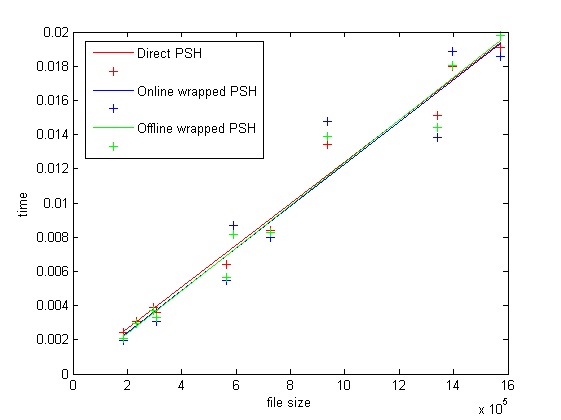
\includegraphics[width = 0.7\textwidth]{./DirectOnlineOffline.png}
	\caption{Performance of our implementation}
	\label{fig:directpoly}
\end{figure}


(figure)

Using the speedup, wrapped polynomial string hashing, we expect a time-improvement compared to the direct string hashing. We use the same example files as above, and obtain a speed-up of cirka . %TODO: hvad er speedup?

(figure)

Since we also implemented our own version of Pair-multiply-shift, we also compare that to the standard library. 

\section{Conclusions and Future Work}

One of the immediate problems present throughout this project, is the fact that neither of us are experienced \cpp programmers, which probably goes some way in explaining the inefficiency of our solution. For example, the

%One direct optimisation in the wrapped PSH would be to only call \funk{reduce}
%once and let it return a 64-bit integer. This 
\end{document}
